% =========================================================================== %
% TeX input file: "Create the hello world backend"
%
% WARNING: this tex file does not compile standalone, it needs to be embedded
% in a master tex document (e.g. Introduction.tex)
% =========================================================================== %

The responsibility of the Scout server in our ''Hello World'' application is to provide an initial text content for the message field in the client's user interface.
We implement this behaviour in the \java{load} method of the server's \java{DesktopService}.
An empty stub for the \java{load} method of the \java{DesktopService} service has already been created during the initial project creation step. 

To navigate to the implementation of the desktop service in the Scout SDK, we first expand the blue top-level \node{server} in the Scout Explorer.
Below the server node, we then expand the \folder{Services} which shows the \element{DesktopService} element.
Expanding this \element{DesktopService} node, the \java{load} method becomes visible as shown in \figref{helloworld_load_servicemethod}.

\begin{figure}
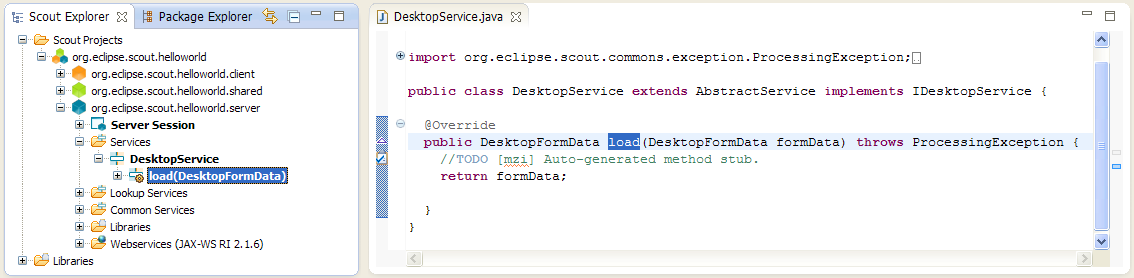
\includegraphics[width=14cm]{sdk_server_desktopservice_load.png}
\caption{The Scout Explorer showing the blue server node expanded with the \folder{Services}.
In this folder the \element{load} method of \element{DesktopService} is selected and its initial implementation is shown in the editor on the right side.}
\figlabel{helloworld_load_servicemethod}
\end{figure}

The \java{DesktopService} represents the server service corresponding to the \java{DesktopForm} on the client side.
This initial setup represents Scout's default where client forms and server services typically come in pairs.
Whenever the client's user interface displays a form to the user, the client connects to the server and calls the \java{load} method of the corresponding server service.
We just need to add our business logic to the \java{load} method of the server's \java{DesktopService}.

According to the signature of the \java{load} method, a \java{formData} object is passed into this method that is then handed back in the return statement.
To complete the implementation of the \java{load} method it is sufficient to assign the text 'hello world!' to the message field part of the form data according to the following line.

\begin{lstlisting}[backgroundcolor=\color{white}]
// test comment
formData.getMessage().setValue("Hello World!");
\end{lstlisting}

The complete implementation of the load method is provided below.
With this last element we have completed the Scout ''Hello World'' application.

\begin{lstlisting}
@Override
public DesktopFormData load(DesktopFormData formData) 
    throws ProcessingException 
{
    formData.getMessage().setValue("Hello World!"); 
    return formData;
}
\end{lstlisting}

% =========================================================================== %
% EOF TeX input file
% =========================================================================== %
